%%%%%%%%%%%%%%%%%%%%%%%%%%%%%%%%%%%%%%%%%%%%%%%%%%%
%
%  New template code for TAMU Theses and Dissertations starting Fall 2016.
%
%
%  Author: Sean Zachary Roberson 
%	 Version 3.16.09
%  Last updated 9/12/2016
%
%%%%%%%%%%%%%%%%%%%%%%%%%%%%%%%%%%%%%%%%%%%%%%%%%%%

%%%%%%%%%%%%%%%%%%%%%%%%%%%%%%%%%%%%%%%%%%%%%%%%%%%%%%%%%%%%%%%%%%%%%%
%%                           APPENDIX A 
%%%%%%%%%%%%%%%%%%%%%%%%%%%%%%%%%%%%%%%%%%%%%%%%%%%%%%%%%%%%%%%%%%%%%

\phantomsection

\chapter{\uppercase{Appendix: Optimization Results Obtained by snapping cuts to the largest jumps }}\label{appendix1}

Figures~\ref{ubp_comp1} and~\ref{ubp_comp2} show the time-to-solution for the binary tree, regular, load-balanced, and load-balanced-by-dimension cuts on the unbalanced pin mesh and ``heavier'' unbalanced pin mesh, respectively.
Figure~\ref{ubp_comp3} shows the Level-2 mesh sweep times from the time-to-solution estimator and PDT for (1) regular cuts, (2) hand-balanced cuts, (3) load-balanced cuts, (4) load-balanced-by-dimension cuts, and (5) binary tree cuts.

\begin{figure}[h]
\centering
  \begin{subfigure}[t]{0.49\textwidth}
    \centering
  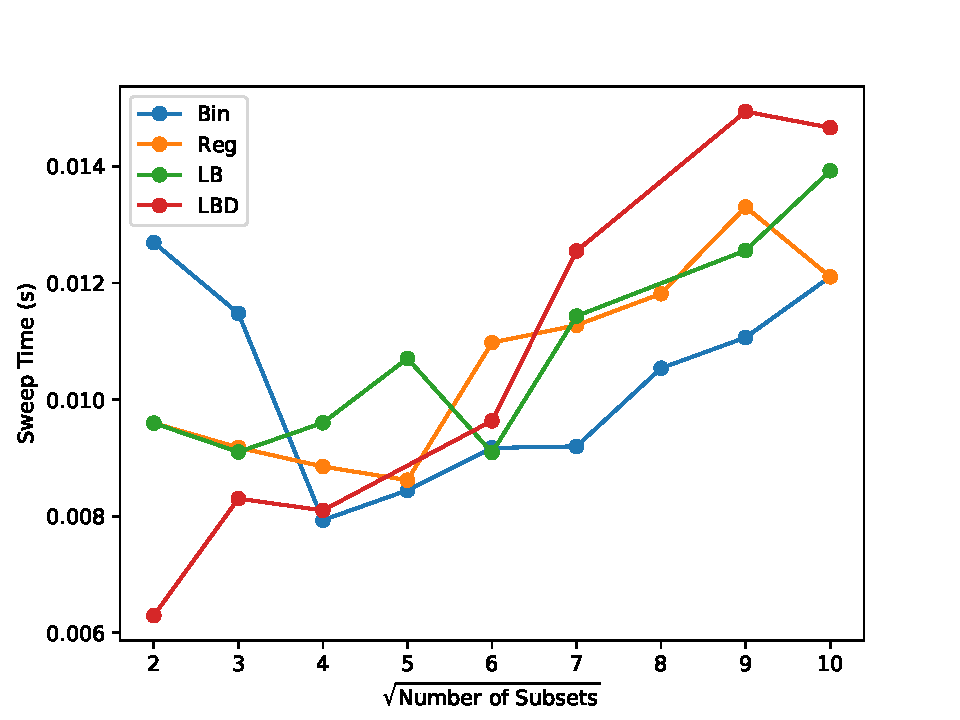
\includegraphics[scale=0.55]{../../figures/unbalanced_pins_opt_comparison.pdf}
  \end{subfigure}
   \begin{subfigure}[t]{0.49\textwidth}
   \centering
   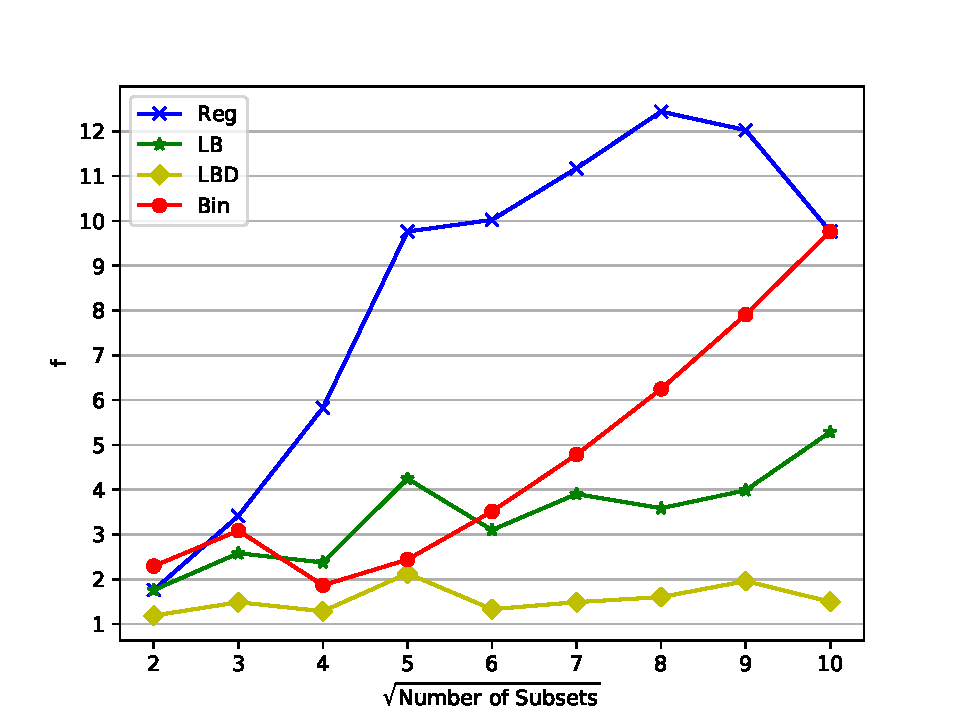
\includegraphics[scale=0.55]{../../figures/spiderweb_metric_study_bad.pdf}
   \end{subfigure}
  \caption{The time-to-solution for binary tree, regular, load-balanced and load-balanced-by-dimension cuts on the unbalanced pins mesh from 2 to 10 subsets in each dimension.}
  \label{ubp_comp1}
\end{figure}
\begin{figure}[h]
\centering
  \begin{subfigure}[t]{0.49\textwidth}
    \centering
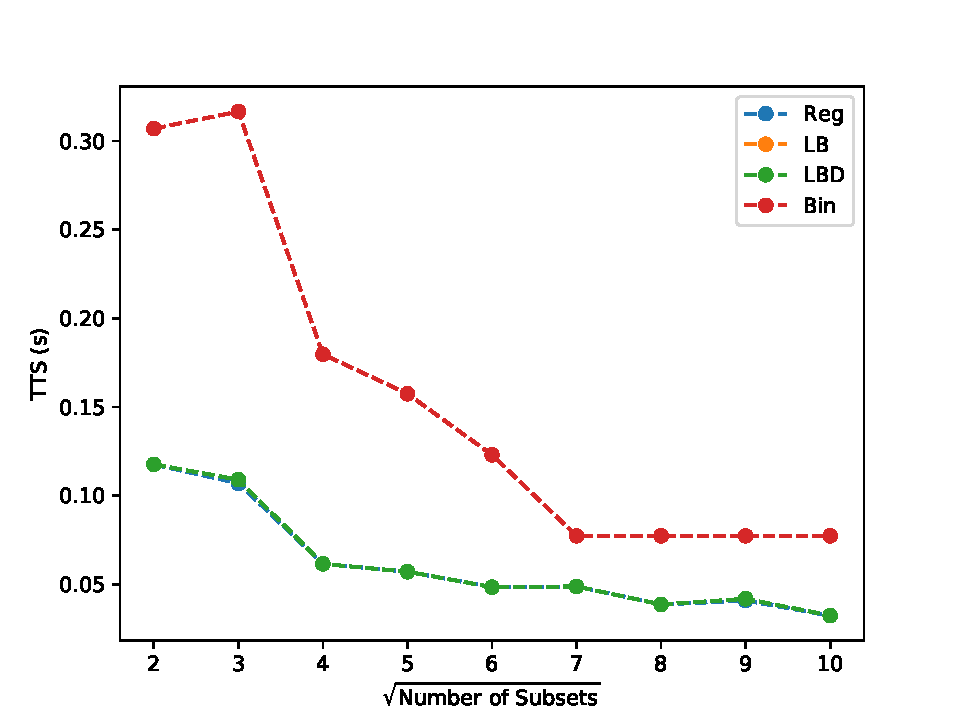
\includegraphics[scale=0.55]{../../figures/more_sparse_comp.pdf}
  \end{subfigure}
  \begin{subfigure}[t]{0.49\textwidth}
    \centering
    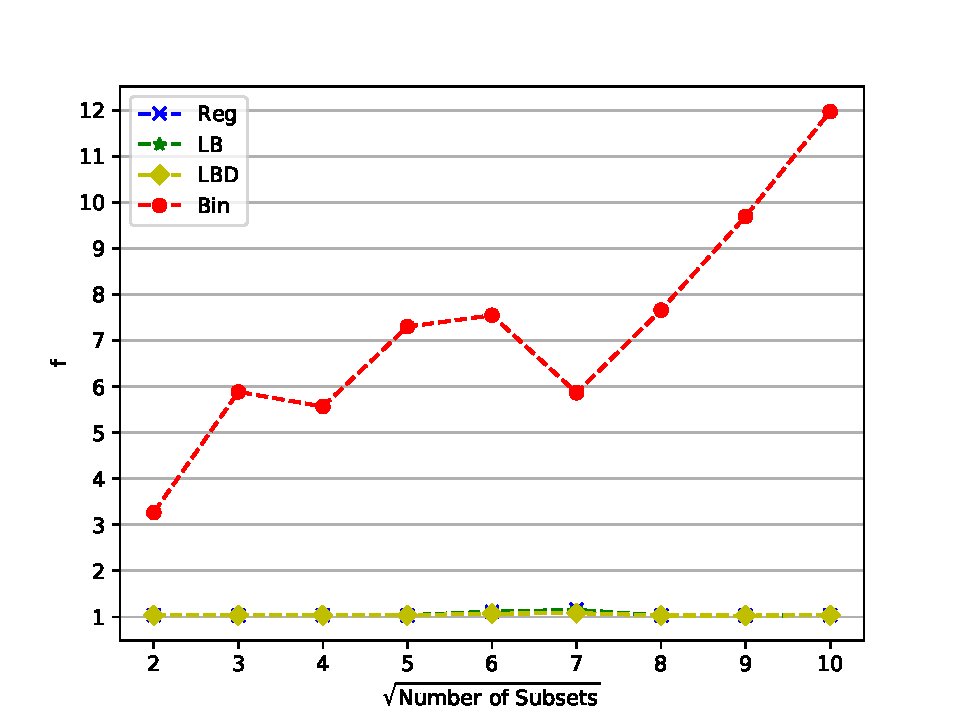
\includegraphics[scale=0.55]{../../figures/more_sparse_metric_comp_bad.pdf}
  \end{subfigure}  
  \caption{The time-to-solution for binary tree, regular, load-balanced and load-balanced-by-dimension cuts on the ``heavier'' unbalanced pins mesh from 2 to 10 subsets in each dimension.}
  \label{ubp_comp2}
\end{figure}
%%%
\begin{figure}[h]
\begin{minipage}[c]{0.65\textwidth}
\centering
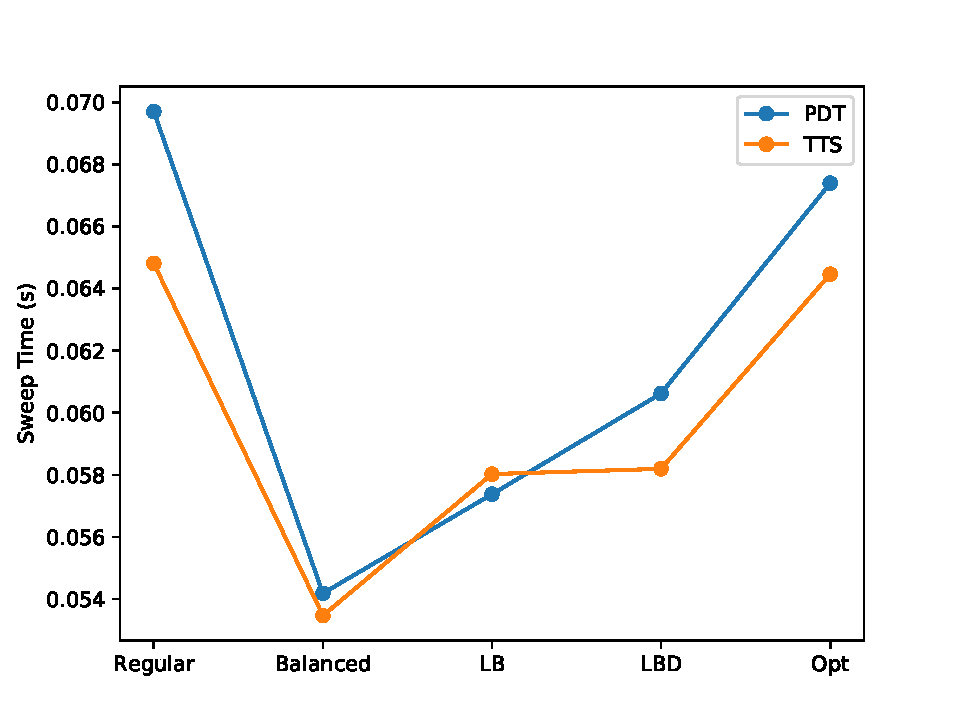
\includegraphics[scale=0.65]{../../figures/level2_sweep_comp.pdf}
\end{minipage}
\begin{minipage}[c]{0.33\textwidth}
\begin{table}[H]
\centering
\begin{tabular}{c|c}
\textbf{Type} & \bf $f$ \\ \hline
Regular &  32.62 \\ \hline
Balanced & 2.38 \\ \hline
LB & 5.01 \\ \hline
LBD &  1.99\\ \hline
Bin. &  21.96 \\ \hline
\end{tabular}
\end{table}
\end{minipage}
\caption{The Level-2 mesh sweep times from the time-to-solution estimator for (1) regular cuts, (2) hand-balanced cuts, (3) load-balanced cuts, (4) load-balanced-by-dimension cuts, and (5) optimized cuts. Additionally, the load-balance metric $f$ is reported for each partition type. }
\label{ubp_comp3}
\end{figure}